% !TEX program = xelatex
%----------------------- Преамбула -----------------------
\documentclass[ut8x, 14pt, oneside, a4paper]{extarticle}

\usepackage{extsizes} % Для добавления в параметры класса документа 14pt

% Для работы с несколькими языками и шрифтом Times New Roman по-умолчанию
\usepackage[english,russian]{babel}
\usepackage{fontspec}
\setmainfont{Times New Roman}

% ГОСТовские настройки для полей и абзацев
\usepackage[left=30mm,right=10mm,top=20mm,bottom=20mm]{geometry}
\usepackage{misccorr}
\usepackage{indentfirst}
\usepackage{enumitem}
\usepackage{pdfpages}
\setlength{\parindent}{1.25cm}
%\setlength{\parskip}{1em} % поменять
%\linespread{1.3}
\renewcommand{\baselinestretch}{1.5}
\setlist{nolistsep} % Отсутствие отступов между элементами \enumerate и \itemize

% Дополнительное окружения для подписей
\usepackage{array}
\newenvironment{signstabular}[1][1]{
	\renewcommand*{\arraystretch}{#1}
	\tabular
}{
	\endtabular
}

% Переопределение стандартных \section, \subsection, \subsubsection по ГОСТу;
% Переопределение их отступов до и после для 1.5 интервала во всем документе
\usepackage{titlesec}

\titleformat{\section}[block]
{\bfseries\normalsize\filcenter}{\thesection}{1em}{}

\titleformat{\subsection}[hang]
{\bfseries\normalsize}{\thesubsection}{1em}{}
\titlespacing\subsection{\parindent}{\parskip}{\parskip}

\titleformat{\subsubsection}[hang]
{\bfseries\normalsize}{\thesubsubsection}{1em}{}
\titlespacing\subsubsection{\parindent}{\parskip}{\parskip}

% Работа с изображениями и таблицами; переопределение названий по ГОСТу
\usepackage{caption}
\captionsetup[figure]{name={Рисунок},labelsep=endash}
\captionsetup[table]{singlelinecheck=false, labelsep=endash}

\usepackage{graphicx}
\usepackage{diagbox} % Диагональное разделение первой ячейки в таблицах

% Цвета для гиперссылок и листингов
\usepackage{color}

% Гиперссылки \toc с кликабельностью
\usepackage{hyperref}

\hypersetup{
	linktoc=all,
	linkcolor=black,
	colorlinks=true,
}

% Листинги
%\setsansfont{Arial}
%\setmonofont{Courier New}

\usepackage{color} % Цвета для гиперссылок и листингов
%\definecolor{comment}{rgb}{0,0.5,0}
%\definecolor{plain}{rgb}{0.2,0.2,0.2}
%\definecolor{string}{rgb}{0.91,0.45,0.32}
%\hypersetup{citecolor=blue}
\hypersetup{citecolor=black}

\usepackage{listings}
\lstset{
	basicstyle=\footnotesize\ttfamily,
	language=[Sharp]C, % Или другой ваш язык -- см. документацию пакета
	commentstyle=\color{comment},
	numbers=left,
	numberstyle=\tiny\color{plain},
	numbersep=5pt,
	tabsize=4,
	extendedchars=\true,
	breaklines=true,
	keywordstyle=\color{blue},
	frame=b,
	stringstyle=\ttfamily\color{string}\ttfamily,
	showspaces=false,
	showtabs=false,
	xleftmargin=17pt,
	framexleftmargin=17pt,
	framexrightmargin=5pt,
	framexbottommargin=4pt,
	showstringspaces=false,
	inputencoding=utf8x,
	keepspaces=true
}

\DeclareCaptionLabelSeparator{line}{\ --\ }
\DeclareCaptionFont{white}{\color{white}}
\DeclareCaptionFormat{listing}{\colorbox[cmyk]{0.43,0.35,0.35,0.01}{\parbox{\textwidth}{\hspace{15pt}#1#2#3}}}
\captionsetup[lstlisting]{
	format=listing,
	labelfont=white,
	textfont=white,
	singlelinecheck=false,
	margin=0pt,
	font={bf,footnotesize},
	labelsep=line
}

\usepackage{ulem} % Нормальное нижнее подчеркивание
\usepackage{hhline} % Двойная горизонтальная линия в таблицах
\usepackage[figure,table]{totalcount} % Подсчет изображений, таблиц
\usepackage{rotating} % Поворот изображения вместе с названием
\usepackage{lastpage} % Для подсчета числа страниц

\makeatletter
\renewcommand\@biblabel[1]{#1.}
\makeatother

\usepackage{color}
\usepackage[cache=false, newfloat]{minted}
\newenvironment{code}{\captionsetup{type=listing}}{}
\SetupFloatingEnvironment{listing}{name=Листинг}

\usepackage{amsmath}
\usepackage{slashbox}


% ---------------------- Документ ----------------------
\begin{document}
\normalsize
\setcounter{page}{3}

\pagebreak

\tableofcontents
\normalsize

\pagebreak

% Хэш-функция --- функция, осуществляющая преобразование массива входных данных произвольной длины в выходную битовую строку установленной длины, выполняемое определенным алгоритмом. \cite{hash}
% Криптографическая стойкость --- способность криптографического алгоритма противостоять криптоанализу. Стойким считается алгоритм, успешная атака на который требует от атакующего обладания недостижимым на практике объемом вычислительных ресурсов либо настолько значительных затрат времени на раскрытие, что к его моменту защищенная информация утратит свою актуальность. \cite{crypto}
% Блокчейн --- выстроенная по определенным правилам непрерывная последовательная цепочка блоков --- элементов, содержащих информацию. \cite{bitcoin}

\section*{ВВЕДЕНИЕ}
\addcontentsline{toc}{section}{ВВЕДЕНИЕ}

Обеспечение защиты от неправомерного доступа --- мера по защите информации. При работе с информацией лицо, имеющее доступ к этой информации, ограничено правами, которые определяют способы взаимодействия с информацией. В качестве примера таких прав можно привести права на чтение, изменение и удаление информации.

Цель работы --- рассмотреть существующие методы хранения информации с защитой от неправомерного доступа.

Для достижения поставленной цели требуется решить следующие задачи:
\begin{itemize}
	\item [---] описать способы защиты информации;
	\item [---] рассмотреть базовые элементы и понятия, используемые при проектировании методов хранения информации с возможностью защиты от неправомерного доступа;
	\item [---] провести анализ существующих методов хранения информации с защитой от неправомерного доступа.
\end{itemize}
\pagebreak

\section{Анализ предметной области}

\subsection{Способы защиты информации}

Задача по обеспечению защиты от неправомерного доступа может решаться на нескольких уровнях:
\begin{enumerate}
    \item Отсутствие возможности неправомерного доступа. Самый желаемый уровень, при котором лицо не имеет возможности превышения прав при работе с информацией. Для чтения, например, может достигаться за счет шифрования данных на диске, где ключ шифрования имеется только у лиц, обладающими правами на чтение.
    \item Наличие возможности устранения последствий неправомерного доступа. Данный уровень может быть использован совместно с исключением неправомерного доступа, обеспечивая дополнительную защиту. Примерами методов защиты, обеспечиваюими описанную возможность, могут послужить резервное копирование и репликация данных.
    \item Наличие возможности доказательства неправомерного доступа. Данный уровень служит для ответа на вопрос, являются ли данные целостностными. Для обеспечения такой возможности может использоваться, например, расчет контрольных сумм.
\end{enumerate}

При этом в общем случае работа с хранилищем данных подразумевает 3 действия:
\begin{enumerate}
	\item [---] чтение;
	\item [---] изменение;
	\item [---] удаление.
\end{enumerate}

Однако данные действия требуется уточнить. При обеспечении защиты на уровне возможности устранения последствий неправомерного доступа восстановление данных при изменении и удалении возможно при наличии в системе избыточной информации об удаленных или измененных фрагментах. Данное условие накладывает некоторые ограничения на операции изменения и удаления. Таким образом для рассматриваемого уровня защиты можно ввести 2 дополнительные неправомерные операции:

\begin{enumerate}
	\item [---] частичное удаление;
	\item [---] частичное изменение.
\end{enumerate}

Стоит также учесть, что меры защиты применимы не ко всем операциям. Например, невозможно устранить последствия неправомерного чтения. С учетом этого и всего вышесказанного можно выделить итоговый список способов защиты информации, которые могут обеспечиваться хранилищем данных:
\begin{itemize}
	\item [---] исключение неправомерного чтения;
	\item [---] исключение неправомерного изменения;
	\item [---] исключение неправомерного удаления;
	\item [---] возможность устраненения последствий частичного неправомерного удаления;
	\item [---] возможность устраненения последствий частичного неправомерного изменения;
	\item [---] доказательство неправомерного удаления;
	\item [---] доказательство неправомерного изменения.
\end{itemize}

\subsection{Базовые понятия}

\subsubsection{Хэш-функция}

Хэш-функция --- функция, осуществляющая преобразование массива входных данных произвольной длины в выходную битовую строку установленной длины, выполняемое определенным алгоритмом. \cite{hash}

Хэш-функции применяются:
\begin{itemize}
    \item[---] при решении задачи дедубликации;
    \item[---] при построении идентификаторов;
    \item[---] при вычислении контрольных сумм;
    \item[---] при хранении паролей.
\end{itemize}

Криптографическая стойкость --- способность криптографического алгоритма противостоять криптоанализу. Стойким считается алгоритм, успешная атака на который требует от атакующего обладания недостижимым на практике объемом вычислительных ресурсов либо настолько значительных затрат времени на раскрытие, что к его моменту защищенная информация утратит свою актуальность. \cite{crypto}

При рассмотрении хэш-функций под алгоритмом подразумевается процесс вычисления значения хэш-функции, а под атакой на алгоритм --- решение обратной задачи: нахождение для заданного значения хэш-функции \textit{H1} такого массива входных данных \textit{A1}, что \textit{f(A1) = H1}. Хэш-функцию, которая является стойкой по определению криптографической стойкости по отношению к такой задаче, называют криптостойкой.

Криптостойкие функции также обладают следующим свойством: при наличии массива входных данных \textit{A1} и значения хэш-функции для него \textit{f(A1)}, настолько же сложной задачей, что и нахождения обратного значения, является задача нахождения такого отличного от \textit{A1} значения массива входных данных \textit{A2}, для которого верно \textit{f(A1) = f(A2)}. Такие значения \textit{A1} и \textit{A2}, для которых верно равенство \textit{f(A1) = f(A2)}, называются коллизиями.

\subsubsection{Блокчейн}

Блокчейн --- выстроенная по определенным правилам непрерывная последовательная цепочка блоков --- элементов, содержащих информацию. \cite{bitcoin} В общем случае такая цепочка поддерживает 2 операции:
\begin{enumerate}
    \item добавление нового элемента в конец цепочки;
    \item проверка целостности всей цепочки.
\end{enumerate}

При добавлении блока вычисляется значения хэша от его содержимого и хэша предыдущего блока. Вычисленное значение считается хэшом добавляемого блока.

Пример блокчейна изображен на рисунке \ref{fig:blockchain}.

\begin{figure}[hbtp]
    \centering
    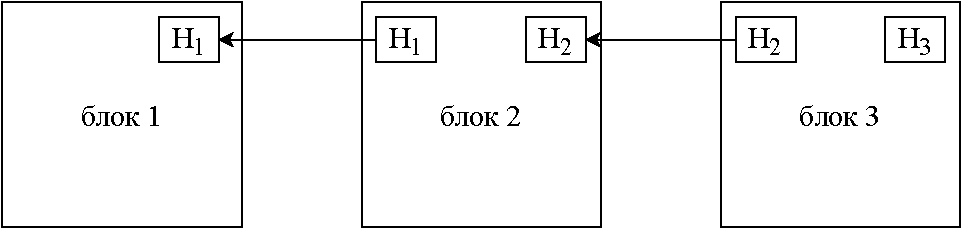
\includegraphics[width=\textwidth]{img/blockchain.pdf}
    \caption{Пример блокчейна}
    \label{fig:blockchain}
\end{figure}

При проверки целостности цепочки выполняются следующие действия:
\begin{enumerate}
    \item Высчитывается хэш от содержимого первого блока и сравнивается со значением хэша, записанным при добавлении данного блока в цепочку. Если значения не совпадают, то констатируется факт нарушения целостности.
    \item Для очередного блока вычисляется значение хэша от его содержимого и хэша предыдущего блока. Вычисленное значение сравнивается со значением хэша, записанным при добавлении блока. При несовпадении констатируется факт нарушения целостности.
\end{enumerate}

При изменении последнего блока достаточно пересчитать и перезаписать значения хэша только для него. Однако при изменении хэша блока, не являющегося последним, потребуется пересчитать значение хэша всех последующих блоков, что в некоторых системах может потребовать больших вычислительных затрат.

\subsubsection{Дерево и ориентированный ациклический граф Меркла}

Дерево Меркла \cite{merkle} --- двоичное дерево, в листовые вершины которого помещены хэши блоков данных, а внутренние вершины содержат хэши суммы значений в дочерних вершинах. В общем случае операция сложения --- произвольная функция от 2 аргументов \textit{f(x, y)}, которая может быть несимметричной (например, конкатенация строк). Корневой узел дерева содержит хэш от всего набора данных, то есть такое дерево является однонаправленной хэш-функцией.

Пример дерева меркла можно увидеть на рисунке \ref{fig:mtree}.

\begin{figure}[hbtp]
    \centering
    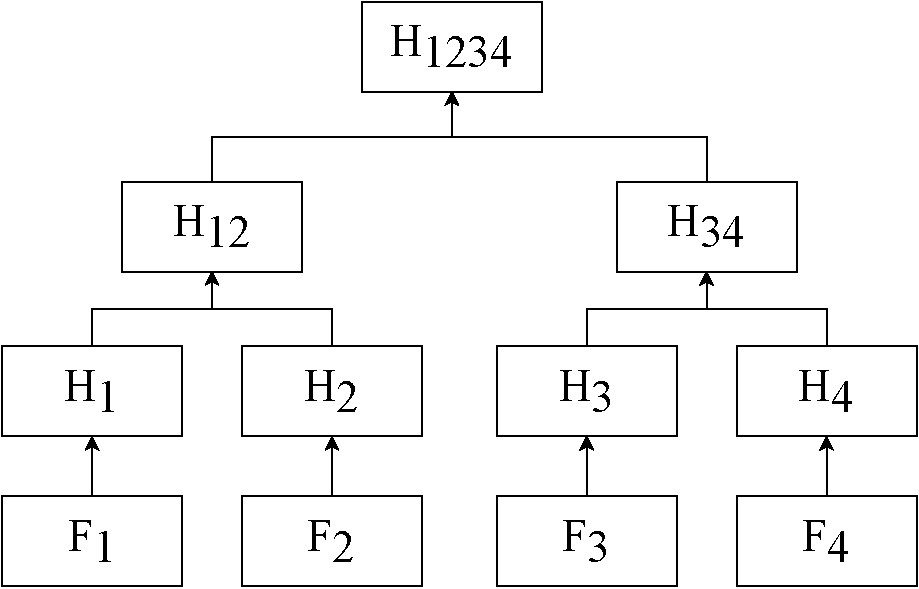
\includegraphics[width=\textwidth]{img/merkletree.pdf}
    \caption{Пример дерева Меркла}
    \label{fig:mtree}
\end{figure}

Применения дерева Меркла:
\begin{itemize}
    \item[---] Хранение транзакций в блокчейне криптовалют (например, в Bitcoin; позволяет получить значение хэша всех транзакций в блоке, а также эффективно верифицировать транзакции).
    \item[---] Для множества значений в среде с ограничением по памяти. В среде хранится только корень дерева. Для проверки принадлежности элемента множеству вместе с элементом требуется передать доказательство Меркла --- значения всех хэшей, с которыми суммируется хэш проверяемого элемента на пути из листа в корень.
\end{itemize}

Ориентированный ациклический граф Меркла \cite{merkledag} --- структура данных, представляющая собой граф, строящийся по следующим правилам:
\begin{enumerate}
    \item Все вершины графа, степень полуисхода \cite{graphs} которых равна 0, представляют хэши данных.
    \item Вычисление значений остальных вершин графа делается в порядке, обратном топологической сортировке \cite{topsort}. Хэшем очередной вершины будет значение хэша от суммы вершин, в которые есть дуга из рассматриваемой вершины.
\end{enumerate}

%
Данная структура данных используется в системе версионного контроля Git \cite{git}.

\section{Существующие решения}

\subsection{PASIS}

\label{par:pasis}

PASIS \cite{pasis} --- распределенное хранилище данных, реализующее метод хранения, защищающий от ошибок, связанных с подменой данных определенными узлами системы, называемыми византийскими. Узлы хранилища хранят данные фрагментами и версионируют информацию. Клиенты читают и пишут фрагменты данных.

Данные клиента распределяются по фрамгентам на \textit{N} узлов хранилища. При чтении данных клиент обращается к \textit{m} узлам, которые являются подмножеством узлов, на которые происходила запись, и проверяет валидность полученных фрагментов. Процесс чтения может быть выполнен в несколько итераций, если в результате валидации будет выявлена ошибка. Процесс чтения считается завершенным, если получено \textit{m} верных фрагментов. Каждый отдельный фрагмент не несет в себе информации, исходные данные можно восстановить только по \textit{m} и большему числу фрагментам.

Данные восстанавливаются из фрагментов с помощью стирающих кодов\cite{erasurecode} и проверяются с помощью объединенных контрольных сумм \cite{pasis}. Объединенная контрольная сумма --- конкатенация хэшей всех \textit{N} записываемых фрагментов. После восстановления данных в наличии у читателя имеются все \textit{N} фрагментов, для которых можно рассчитать значение хэша и проверить подлинность данных.

Таким образом использование данной системы позволяет защититься от неправомерного изменения или удаления данных на части узлов хранилища с возможностью восстановления данных, а также доказать неправомерное изменение данных.

\subsection{Криптографические файловые системы}

В отличие от обычных файловых систем, криптографические файловые системы имеют дополнительный слой между виртуальной файловой системой и драйвером файловой системы, который шифрует данные. При такой реализации работа слоя шифрования данных будет прозрачна для пользователя, потому что пользователь работает с виртуальной файловой системой.

TCFS \cite{tcfs}, NCryptFS \cite{ncryptfs} --- примеры криптографических файловых систем.

TCFS использует стандартные для файловых систем способы подключения в ОС \texttt{Linux}: системные вызовы \texttt{mount}, \texttt{ioctl} \cite{linux}. При работе в пределах смонтированной файловой системы все операции записи и чтения проходят через слой шифрования, поэтому данные записываются на устройство только в зашифрованном виде.

NCryptFS обладает похожим принципом работы, однако подключается с помощью собственной команды \texttt{attach}, не используя стандартные методы, и имеет возможность создания пространства имен для управления правами групп пользователей на доступ к определенным директориям, а также содержит средства авторизации.

Описанные системы решают задачу защиты от неправомерного чтения. При случайной записи данных на устройство будет нарушена их целостность, проверка целостности возлагается на приложения, использующие данные файловые системы, но, так как данные хранятся в зашифрованном виде, целостность исходных данных может быть нарушена более значительно. Возможности восстановления данных нет.

\subsection{OceanStore}
\label{par:ocean}

OceanStore \cite{ocean} --- безопасная распределенная read-only файловая система.

Данное хранилище хранит данные в одноранговой сети, где узлы соединены между собой по принципу точка-точка. Преимуществом данного хранилища является хранение данных по фрагментам с использованием стирающих кодов. Данный подход, как уже было показано в \ref{par:pasis}, позволяет получать исходные данные, записанные как \textit{N} фрагментов, из любых \textit{m} фрагментов, где $m < N$.

В данной системе используется понятие самопроверяющихся данных \cite{selfverify}: данные адресуются по идентификатору GUID, который является хэшем от содержимого. Данный хэш считается из дерева Меркла, изображенного на рисунке \ref{fig:ocean}. Каждый фрагмент, помимо самих данных, содержит в себе также доказательство Меркла. При восстановлении данных проверяется каждый фрагмент по отдельности (с помощью доказательства Меркла), а также все данные целиком. Порядок действий можно описать следующим образом:
\begin{enumerate}
    \item Получить \textit{m} фрагментов, проверив у каждого доказательство Меркла.
    \item Восстановить \textit{N} фрагментов с использованием стирающих кодов.
    \item Восстановить данные из \textit{N} фрагментов. % (более сложная операция, чем конкатенация строк в общем случае)
    \item Построить дерево Меркла и убедиться в равенстве корня дерева и GUID.
\end{enumerate}

\begin{figure}[hbtp]
    \centering
    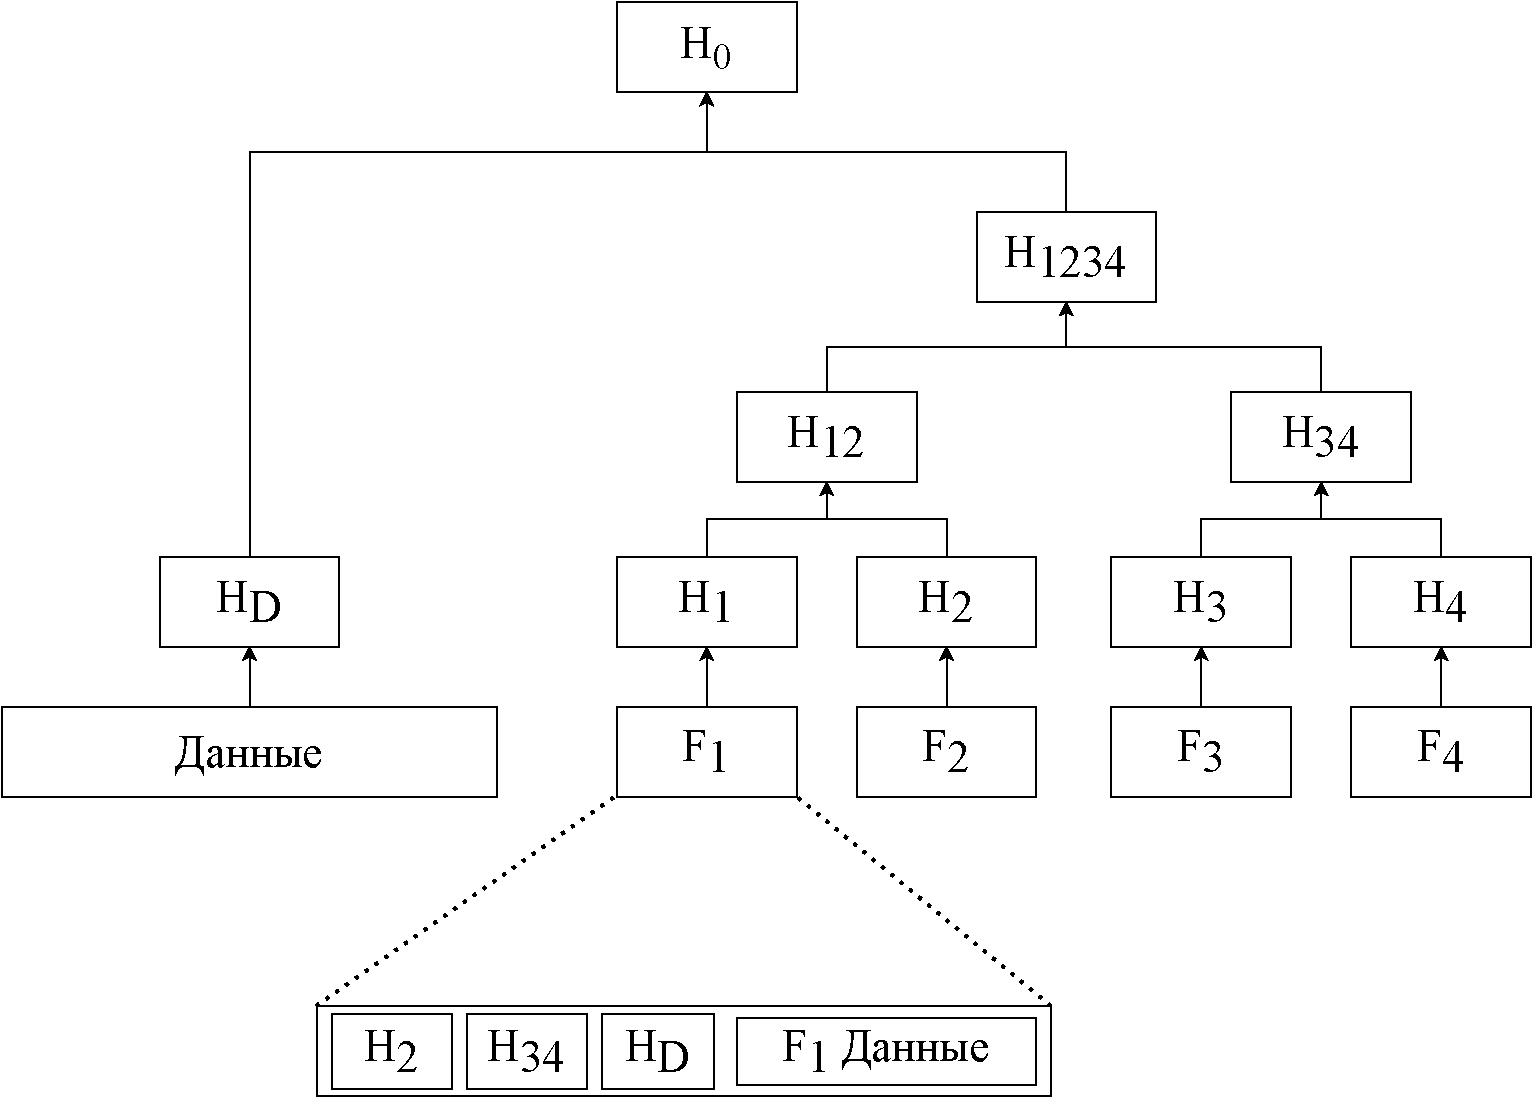
\includegraphics[width=\textwidth]{img/ocean.pdf}
    \caption{Пример дерева Меркла и фрагментов для OceanStore.}
    \label{fig:ocean}
\end{figure}

Данная система считается read-only, потому что изменение данных без изменения идентификатора невозможно, так как идентификатор создается на базе содержимого. Таким образом, например, при обновления версии каких-то данных, старая версия остается неизменной, но появляется новая версия с новым содержимым и GUID.

Данное хранилище, несмотря на внутренее устройство, поддерживает возможность иерархической структуры данных. Для этого требуется в некоторых объектах, которые не являются листьями дерева иерархии данных, хранить хэши дочерних вершин. GUID корня иерархической структуры известен.

На примере иерархической структуры видна сложность изменения данных: изменение элемента дерева приводит к необходимости изменения (замены на новый элемент) всех вершин-предков.

Как и хранилище из раздела \ref{par:pasis}, данная система защищена от частичного удаления или изменения данных, обладает возможностью восстановления, а также обладает возможностью доказательства изменения данных.

\subsection{Git}

Git \cite{git} --- система контроля версий. Данная система не решает задачу защиты от неправомерного доступа непосредественно, однако делает это косвенно: при нарушении целостности данных система перестанет работать, что будет являться доказательством неправомерного доступа. Внутреннее представление Git --- хранилище, адресующее по содержанию. Это означает, что файлы, которыми оперирует Git в рамках системной файловой системы, хранятся в виде ассоциативного массива, доступ в котором осуществляется по ключу. Данная система называется Object Store. В качестве ключа файла выступает хэш от его содержимого, подобно GUID в \ref{par:ocean}.

Иерархическую структуру файлов Git поддерживает в виде ориентированного ациклического графа Меркла за счет наличия 3 основных типов объектов:
\begin{enumerate}
    \item blob --- содержит информацию о конкретной версии файла. В ациклическом графе Меркла файлы этого типа всегда обладают нулевой степенью полуисхода, то есть их хэш составлен на основе содержимого файла. Этим же хэшем данные файлы адресуются в упомянутом выше ассоциативном массиве.
    \item tree --- содержит информацию о конкретной версии директории. Данный объект содержит в себе другие объекты (больше 0), которые могут быть типа blob или tree. Он обладает отличной от обычной функцией суммирования: вместо простой конкатенации хэшей вершин, в которые ведут дуги, в функции суммирования также фигурируют имена файлов дочерних вершин (реальные имена, не хэши), а также режимы доступа к данным файлам.
    \item commit --- содержит информацию о коммите --- фиксированном состоянии системы. commit обладает единичной степенью полуисхода и единственная его дуга ведет в объект типа tree, соотвествующей корневой директории репозитория. Объект типа commit хранит информацию об авторе изменений, связанных с коммитом, об имени, хэше и режиме доступа корневой директории и информацию о хэше родительского коммита --- то есть предыдущей зафиксированной версии. Адресуется коммит значением хэш функции от его содержимого. Схема, по которой описанный коммит связан с предыдущим, в точности соответствует схеме работы блокчейна.
\end{enumerate}

На рисунке \ref{fig:git1} схематично представлен пример графа для 3 основных типов объектов.

\begin{figure}[hbtp]
    \centering
    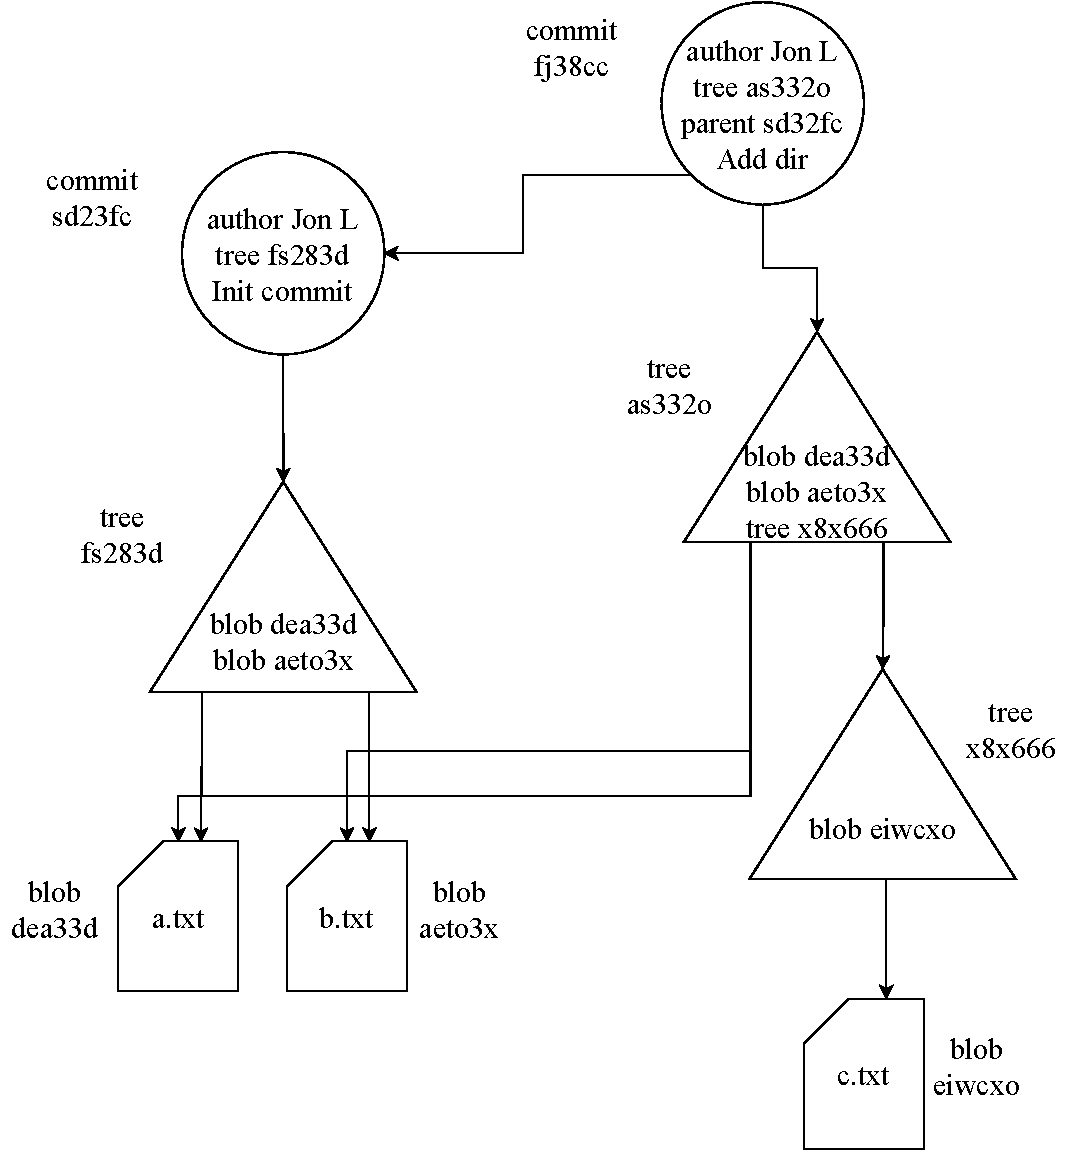
\includegraphics[width=\textwidth]{./img/git-mdag.pdf}
    \caption{Пример графа Меркла для 3 основных типов объектов}
    \label{fig:git1}
\end{figure}

Изменение внутренней структуры в процессе изменения данных происходит в 3 этапа:
\begin{enumerate}
    \item Изначально Git не будет учитывать изменения в рабочей директории, то есть при изменении файла у системы будет иметься копия файла из рабочей директории, которая не будет изменена.
    \item Чтобы система учла изменения, требуется добавить измененные файлы в индекс. Данное действие приведет к изменению файла с точки зрения файловой системы, с точки зрения внутреннего состояния системы Git это приведет к созданию нового объекта типа blob в Object Store, а также виртуального объекта типа tree (данный объект не будет виден в Object Store на этом этапе). Возможное состояние системы на этом этапе изображено на рисунке \ref{fig:git2}.
    \item При фиксации изменений виртуальный объект типа tree, соответствующий корню рабочей директории для новых версий файлов, добавленных в индекс, становится реальным, то есть создается объект в Object Store, а также создается объект типа commit, который ссылается (содержит хэш в качестве значения) на вновь созданный объект типа tree. Возможное состояние после всех проделанных действий изображено на рисунке \ref{fig:git3}.
\end{enumerate}

\begin{figure}[hbtp]
    \centering
    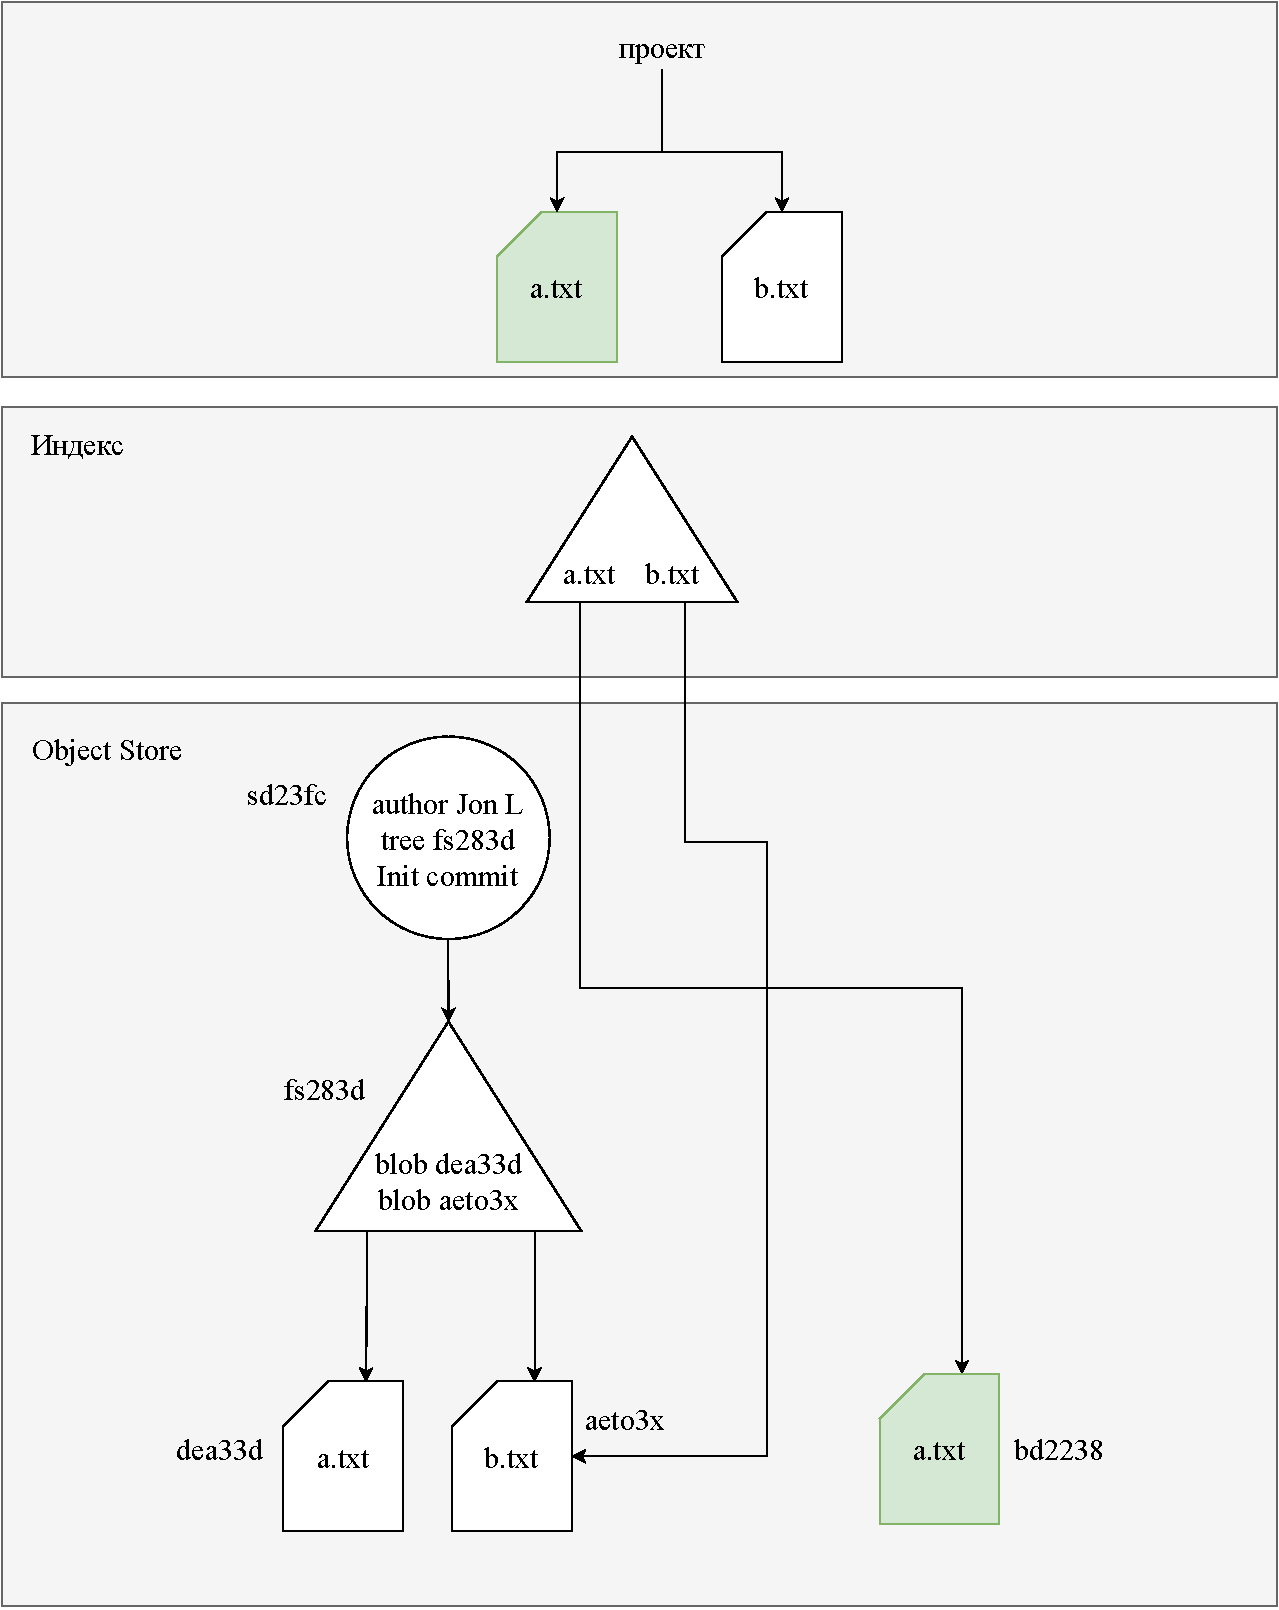
\includegraphics[width=\textwidth]{./img/git-add.pdf}
    \caption{Возможное состояние системы контроля версий Git при добавлении нового файла в индекс.}
    \label{fig:git2}
\end{figure}

\begin{figure}[hbtp]
    \centering
    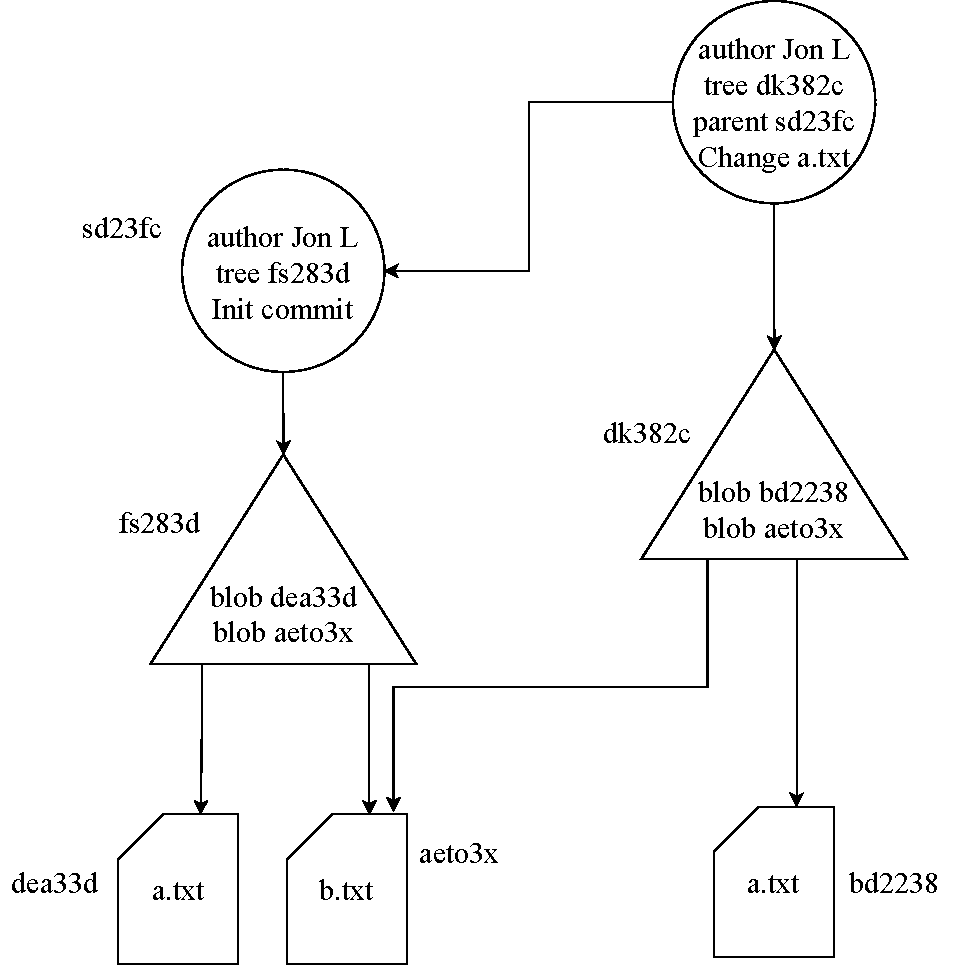
\includegraphics[width=\textwidth]{./img/git-commit.pdf}
    \caption{Возможное состояние системы контроля версий Git после фиксирования изменений.}
    \label{fig:git3}
\end{figure}

Неправомерный доступ подразумевает возможность доступа на запись к внутренней структуре, изменения в которой происходят исключительно за счет добавления новых объектов.

Возможны 3 варианта:
\begin{enumerate}
    \item Изменение содержимого объекта. Имя файла в системе Git --- его хэш и любое изменение содержимого приведет к несовпадению рассчитываемого хэша и имени файла, что приведет к ошибке и обнаружению нарушения в данных.
    \item Удаление объекта. Такая атака будет обнаружена в момент, когда произойдет попытка обращения к удаленному файлу. Он не будет найден в Object Store и будет ошибка.
    \item Добавление объекта. Добавление объекта не будет обнаружено, однако и данные, добавленные с новым объектом, не будут использованы ввиду того, что никакой другой объект не будет ссылаться на вновь созданный. Если добавить коммит в конце цепочки, то появляется возможность посчитать хэш вместе с хэшем предыдущего commit объекта, однако подобный формат работы похож на стандартный и может быть осуществлен извне.
\end{enumerate}

Таким образом данная система обладает возможностью доказательства неправомерного изменения, а также удаления. Однако в общем случае возможно пересчитать значения хэшей, на которые влияет изменение или удаление, что приведет к потере возможности доказательства.

\clearpage

\subsection{Bitcoin}

Bitcoin \cite{bitcoin} --- одноранговая децентрализованная электронная денежная система.

Для данной системы недопустимы сценарии, при которых данные теряются и приводится только доказательство неправомерного доступа к данным. Ввиду того, что данная система является распределенной, у нее нет единого состояния, что усложняет получение неправомерного доступа к данным и их изменение или повреждение без возможности восстановления.

Транзакция --- операция передачи биткойнов с одного адреса на другой. Транзакция осуществляется следующим образом:

\begin{enumerate}
    \item Владелец биткойн-адреса (который связан с публичным ключом) использует любую совершенную транзакцию, в которой адресом назначения является данный адрес.
    \item Создается новая транзакция, которая содержит информацию о наборе адресов и соответсвующем количестве биткоинов, которые требуется перевести в рамках транзакции.
    \item Данная транзакция подписывается приватным ключом владельца кошелька, с которого происходит передача биткоинов.
\end{enumerate}

Таким образом невозможность неправомерного изменения транзакции обеспечивается за счет PKI \cite{pki}.

Транзакция является составным элементом блока. Блок --- составленный по определенным правилам набор транзакций.

Блок имеет определенную структуру, в которую входят:
\begin{itemize}
    \item[---] магическое число;
    \item[---] размер блока;
    \item[---] заголовок блока;
    \item[---] счетчик транзакций;
    \item[---] набор транзакций.
\end{itemize}

Заголовок блока состоит из следующих полей:
\begin{itemize}
    \item[---] версия блока;
    \item[---] хэш заголовка предыдущего блока;
    \item[---] хэш корня дерева Меркла, составленного из транзакций, входящих в данный блок;
    \item[---] текущее время;
    \item[---] целевое значение хэша, ниже которого должен быть хэш от заголовка;
    \item[---] число \textit{Nonce}, которое подбирается таким образом, чтобы хэш от заголовка был меньше целевого значения.
\end{itemize}

Блоки образуют блокчейн --- в заголовке очередного блока содержится хэш предыдущего блока, с помощью которого блоки собираются в цепь. Из одного блока может исходить несколько других блоков, которые содержат первый, как предшествующий. Действующей цепочкой считается наиболее длинная. В этом смысл концепции, называемой proof-of-work: большинство пользователей берут наиболее длинную цепочку блоков и коллективно пытаются подобрать требуемое значение \textit{Nonce}, которое бы удовлетворяло условию целевого значения, тем самым концентруя вычислительные мощности и не давая другим цепочкам стать длиннее текущей. Наиболее быстро будет рассчитываться та цепочка, для расчета которой используется наибольшее количество мощностей.

Сложность расчета значений \textit{Nonce} контролируется за счет изменения целевого значения хэша. Можно дать вероятностную оценку сложности вычисления нужного значения хэша в количестве попыток, исходя из следующих условий:
\begin{itemize}
    \item[---] значение хэш функции является случайным значением;
    \item[---] число ведущих нулей в бинарном представлении целевого значения равняется числу $M$.
\end{itemize}

Тогда вероятность появления такого значения хэша, которое будет меньше целевого значения, равна вероятности выпадения $M$ первых нулей при расчете хэша и рассчитывается по формуле \ref{eq:pnce}.

\begin{equation}
    \label{eq:pnce}
    P = \frac{1}{2^M},
\end{equation}

С учетом независимости расчетов для различных $Nonce$ и формулы \ref{eq:pnce}, можно рассчитать количество попыток, требуемых совершить в среднем для получения одного удовлетворяющего числа по формуле \ref{eq:enonce}.

\begin{equation}
    \label{eq:enonce}
    N = \frac{1}{\frac{1}{2^M}} = 2^M,
\end{equation}

Наиболее известный способ атаки на системы, работающие по концепции proof-of-work --- атака 51\%. Суть атаки заключается в том, что атакующий владеет большинством вычислительных мощностей и делает следующие действия:
\begin{enumerate}
    \item Сделать блок, который будет содержать некоторую транзакцию $T_1$.
    \item Дождаться, пока система, на счет которой мы перевели биткоины, будет считать транзакцию $T_1$ завершившейся.
    \item Взять блок, предшествующий блоку из пункта 1, и начать делать новую цепочку без транзакции $T_1$ до тех пор, пока она не станет действующей.
\end{enumerate}

Такая атака позволяет неправомерно изменить данные.

\pagebreak

\section*{ЗАКЛЮЧЕНИЕ}
\addcontentsline{toc}{section}{ЗАКЛЮЧЕНИЕ}

Сравнение рассмотренных методов хранения данных с возможностью защиты от неправомерного доступа можно увидеть в таблице \ref{tab:res}. Обозначения:
\begin{itemize}
    \item[---] НД --- неправомерное действие;
    \item[---] КФС --- криптографические файловые системы;
    \item[---] ЧУ --- частичное удаление;
    \item[---] УЗ --- уровень защиты;
    \item[---] ЧИ --- частичное изменение.
\end{itemize}

Полученные результаты можно свести к следующему:
\begin{itemize}
    \item[---] Защита от чтения возможна в системе, в которой определенная группа людей обладает некоторым уникальным знанием (ключ в КФС).
    \item[---] Восстановление данных после частичного изменения или удаления возможно в распределенных системах, использующих стирающий код, в связи с тем, что фрагменты хранятся в разных местах и допускается неправомерный доступ в части мест.
    \item[---] Исключает возможность полного неправомерного изменения или удаления только Bitcoin, потому что во всех рассмотренных системах количество узлов, в которых хранятся данные, конечно и задано наперед (хоть и в теории может быть очень велико), в то время как в Bitcoin все узлы системы содержат общее состояние.
    \item[---] Возможностью доказательства неправомерного изменения обладают все системы кроме КФС, используя для этого контрольные суммы и хэши. Однако также как в случае удаления, в локальной системе без шифрования нарушитель может восстановить целостность цепочки блоков при изменении внутреннего состояния Git.
    \item[---] Возможностью доказательства неправомерного удаления обладают 2 системы, в основе которых лежит блокчейн. Однако если данные не шифруются никаким образом, то в случае с Git человек, нарушающий права, способен повторить действия самой системы, и произвести изменения, поддержав целостность цепочки блоков.
    \item[---] исключить удаление 
\end{itemize}

\begin{table}[h]
    \begin{center}
        \caption{\label{tab:res} Методы хранения и обеспечиваемая защита.}
        \begin{tabular}{|c|c|c|c|c|c|}
            \hline
            \bfseries НД (УЗ) & \bfseries PASIS & \bfseries КФС & \bfseries OceanStore & \bfseries Git & \bfseries Bitcoin  \\
            \hline
            чтение (исключение) & - & + & - & - & - \\ \hline
            ЧУ или ЧИ (восстановление) & + & - & + & - & - \\ \hline
            изменение (исключение) & - & - & - & - & + \\ \hline
            удаление (исключение) & - & - & - & - & + \\ \hline
            изменение (доказательство) & + & - & + & +/- & + \\ \hline
            удаление (доказательство) & - & - & - & +/- & + \\ \hline
        \end{tabular}
    \end{center}
\end{table}

\clearpage

\section*{СПИСОК ИСПОЛЬЗОВАННЫХ ИСТОЧНИКОВ}
\addcontentsline{toc}{section}{СПИСОК ИСПОЛЬЗОВАННЫХ ИСТОЧНИКОВ}

\begingroup
\renewcommand{\section}[2]{}
\begin{thebibliography}{}
	\bibitem{hash}
	Брюс Шнайер. <<Прикладная криптография. 2-е издание. Протоколы, алгоритмы и исходные тексты на языке С>>.
	\bibitem{crypto}
	Мао В. <<Современная криптография: Теория и практика>> — М.: Вильямс, 2005. — 768 с.
	\bibitem{bitcoin}
	Bitcoin: A Peer-to-Peer Electronic Cash System [Электронный ресурс]. – Режим доступа: 
	https://bitcoin.org/bitcoin.pdf
	свободный – (15.09.2021).
	\bibitem{merkle}
	R.C. Merkle, <<Protocols for public key cryptosystems>>, In Proc. 1980 Symposium on Security and Privacy, IEEE Computer Society, pages 122-133, April 1980.
	\bibitem{merkledag}
	Merkle Directed Acyclic Graphs (DAGs) [Электронный ресурс]. – Режим доступа: 
	https://docs.ipfs.io/concepts/merkle-dag/
	свободный – (17.09.2021).
	\bibitem{graphs}
	Дистель, Рейнхард (2005), <<Graph Theory (3rd ed.)>>, Berlin, New York: Springer-Verlag.
	\bibitem{topsort}
	Левитин А. В. <<Глава 5. Метод уменьшения размера задачи: Топологическая сортировка // Алгоритмы. Введение в разработку и анализ>> — М.: Вильямс, 2006. — С. 220—224. — 576 с.
	\bibitem{git}
	Git Internals --- Git Objects [Электронный ресурс]. – Режим доступа: 
	https://git-scm.com/book/en/v2/Git-Internals-Git-Objects
	свободный – (28.09.2021).
	\bibitem{pasis}
	G. Goodson, J. Wylie, G. Ganger, and M. Reiter, <<Efficient Byzantine-tolerant Erasure-coded Storage>>, Proceedings of the International Conference on Dependable Systems and Networks (DSN-2004). Florence, Italy, 2004. Supercedes Carnegie Mellon University Parallel Data Lab Technical Report CMU-PDL-03-104, December 2003
	\bibitem{erasurecode}
	Dave K. Kythe, Prem K. Kythe. <<Algebraic and Stochastic Coding Theory.>> — 1-е изд. — CRC Press, 2012. — С. 375—395. — 512 с.
	\bibitem{tcfs}
	G.Cattaneo, L. Catuogno, A. Del Sorbo, and P. Persiano, <<A Transparent Cryptographic File System for Unix>>, In Proceedings of the USENIX Annual Technical Conference, Freenix Track. Boston, MA, 2001.
	\bibitem{ncryptfs}
	C. Wright, M. Martino, and E. Zadok. <<NcryptFS: A Secure and Convenient Cryptographic File System>>, In Proceedings of the USENIX Conference General Track, San Antonio, TX, June 2003.
	\bibitem{linux}
	Уорд Б. Внутреннее устройство Linux. — СПб.: Питер, 2016. — 384 с.
	\bibitem{ocean}
	J. Kubiatowitz, D. Bindel, Y. Chen, S. Czerwinski, P. Eaton, D. Geels, R. Gummadi, S. Rhea, H. Weatherspoon, W. Weimer, C. Wells, and B. Zhao, <<Oceanstore: An Architecture for Global-Scale Persistent Storage>>, In Proceedings of the Ninth International Conference on Architectural Support for Programming Languages and Operating Systems, Cambridge, MA, Nov 2000.
	\bibitem{selfverify}
	H. Weatherspoon, C. Wells, and J. Kubiatowicz, <<Naming and Integrity: Self-Verifying Data in Peer-to-Peer Systems>>, In Proceedings of the International Workshop on Future Directions in Distributed Computing (FuDiCo 2002), June 2002.
	\bibitem{pki}
	Полянская О. Ю., Горбатов В. С. <<Инфраструктуры открытых ключей. Учебное пособие.>>, Москва, 2007.
\end{thebibliography}
\endgroup

\pagebreak
\end{document}